\section{Process' Perspective}

\subsection{Team}
To organize our team, we make a weekly plan each Tuesday. The plan depends on the current hangups of the project and the new tasks of the week. \newline
We split up the team in appropriately sized subgroups, depending on the complexity of the task we are taking on.
Each subgroup starts their work immediately and coordinates freely until next week. During the week, we use our Discord server to keep each other updated on progress with the tasks.


\subsection{CI/CD}
%\textcolor{red}{A complete description of stages and tools included in the CI/CD chains. That is, including deployment and release of your systems.}

We have implemented CI/CD with CircleCI. Our CircleCI's configuration includes a list of jobs. Those jobs are: static analysis, build, deploy, and workflows.

In our continuous integration chain, we use different tools to ensure the quality of our extensions to the system.
\begin{itemize}
    \item For static analysis we use a tool called \texttt{golangci-lint}, which runs the following linters in parallel:
    \begin{itemize}
        \item \texttt{gosec} is a tool to enhance security by inspecting the source code for vulnerabilities, by scanning the Go AST.
        \item \texttt{gofmt} is a tool which formats the Go source code, such that for example, unnecessary parenthesis are removed etc. basically functioning as a beautifier (it just runs \texttt{gofmt} command)
        \item \texttt{staticcheck} is a tool which, by using static analysis, is able to locate bugs and find performance issues, while offering simplification and enforcement of style rules.
        \item \texttt{gosimple} is a tool, whose purpose solely is to simplify the source code.
        \item \texttt{unused} is a tool to ensure that unused variables, functions constants and types are removed.
        \item \texttt{typecheck} is a tool, which ensures that our variables are of the correct types.
    \end{itemize}
    \item Quality assessment systems
    \begin{itemize}
        \item Reliability - Static analysis tools (described above) are used to ensure reliability within our system.
        \item Maintainability - We have written our code in a way that makes it easy to read. For example, instead of doing fancy one-liners, we usually write out the code in longer form for better readability, and we also use easy to understand variable names. This makes the code less messy and easier to maintain.
        \item Testability - We didn't have time to translate the Python unit tests, that we were provided, to Go, so we don't have any tests for our code. However, when pushing code to the main branch, CircleCI builds our Docker images, so one could argue that the build is a form of testing.
        \item Portability - It is hard to measure since we have not made use of unit testing or integration testing. What we have to state that our code is somewhat portable is the fact that we use static analysis tools to ensure coding standards and clean conventions.
        \item Reusability - We have reusable code within our application and have made use of reusable code rather than redundant code. An example is our controller, which has methods used by both our API and app.
        % \item During the course of developing and maintaining Minitwit, we tried to minimize our accrued technical debt. To combat it, we kept a backlog of 
        
        %As with all projects, we did not manage perfectly. Having to release on Github
    \end{itemize}    
\end{itemize}


The final step of our CI/CD chain is that we have a Discord bot set up that publishes a message to our Discord server, whenever there is a new commit to the repository. This way, all developers are encouraged to stay up to date with the code base.

\subsection{Repositories}
%\textcolor{red}{Organization of your repositor(ies). That is, either the structure of of mono-repository or organization of artifacts across repositories. In essence, it has to be be clear what is stored where and why.}
We chose to use a mono-repository structure hosted on a single GitHub repository. The repository  includes all of our code for both the API as well as the MiniTwit application. 
We chose to keep the API and application in the same repository since they are both quite small systems, and because they share several dependencies and functions.


\subsection{Branching strategy}
Our branching strategy is based on the trunk-based development process.
We have a main branch which contains a state of our application that works. Whenever we want to make a new feature or fix a bug, we create a new branch from our main branch where we work on the feature. When the work is done, we make a pull request from the work branch into our main branch which then needs to be approved by another team member before it gets merged into main.

\subsection{Development process}
%\textcolor{red}{Applied development process and tools supporting it. For example, how did you use issues, Kanban boards, etc. to organize open tasks}
We add issues to our Github, following the courses weekly additions to the project. All individual issues are added to a To Do List, that tracks their completion. This is to create a quick overview of our progress with the project and keep a backlog.
For weekly tasks, we post a message on our discord, that tracks who is responsible for what.


\subsection{Monitoring}\label{Monitoring}
%\textcolor{red}{How do you monitor your systems and what precisely do you monitor?
%Monitoring..
%Stats fra deres API...}

To monitor our application, we use the tool Prometheus that monitors the metrics we want to track. 
We use the package PromAuto to setup the metrics we want to track with Prometheus. The constructors in PromAuto, in contrast to the Prometheus package, returns \textit{Collectors} that are already registered to a registry. It creates functions on 2 levels: top level functions, that return \textit{Collectors} registered to the global registry, and Factory type methods that returns \textit{Collectors} that are registered with the constructor, that the factory were created with.
\newline
We have chosen to track three metrics. We track them for our App as well as our API. The chosen metrics are
\begin{itemize}
    \item The CPU load
    \item The total number of processed HTTP requests
    \item The average duration of requests
\end{itemize}


To visualize our data, we use the tool Grafana which uses the Prometheus data and visualizes it to us through a web endpoint.

The Grafana dashboard can be seen at the appendix \textit{figure 8} \ref{appendix:dashboard}. The Dashboard makes a nice visual of the chosen metrics and generates an easy overview.

\subsection{Logging}
%\textcolor{red}{What do you log in your systems and how do you aggregate logs?}
We use the ELK stack for logging. The information we log includes:

\begin{itemize}
    \item Caddy access/error logs
    \item App and API error messages
    \item Log messages from the ELK components themselves
\end{itemize}

The log data is read directly from the directory that contains the logs from the Docker containers, which is mounted as a Docker volume on the Filebeat container. Filebeat then parses the data and sends it to Elasticsearch over an internal network connection. The web-frontend we use to look at our logs is Kibana.




\subsection{Security}
%\textcolor{red}{Brief results of the security assessment.}
To estimate the security standing of our system, we sat down as a team and completed a security assessment. We started by doing a risk identification. We concluded that our assets include the user data stored on our servers as well as the web application with almost constant uptime. The related threat sources would thus be unauthorized access to sensitive data, and infrastructure provider downtime that would make our service unavailable. We visualized these risk factors in a risk matrix (see figure \ref{fig:Risk_matrix}) based on their impact and how likely they are to happen.

\begin{figure}[H]
    \centering
    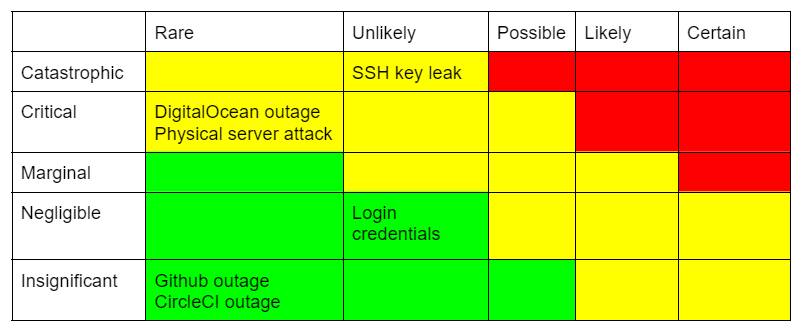
\includegraphics[scale=0.85]{images/risk_matrix.png}
    \caption{The Risk matrix visualizes threats based on their severity and likelihood}
    \label{fig:Risk_matrix}
\end{figure}

The most crucial risk of provider downtime is DigitalOcean, since we host our application with them, which is why we assess downtime on their end as much more crucial than downtime on Github or CircleCI.
\newline
In relation to keeping sensitive user data safe, we identified multiple possible risks scenarios.
The first risk is a physical server attack on DigitalOcean. Since we cannot improve security on their end, the best course of action is to have another provider setup ready. Our personal risk factors are leaked login credentials or an SSH key leak. To improve the security, we have implemented two-factor authentication.


%We have a private ssh key on a physical usb drive that is hacker proof

After pentesting our system with Zaproxy, we found out that we had a number of vulnerabilities, although none of them were too high of a risk. 
One of the medium-risk issues that Zaproxy found was regarding some missing HTTP headers. We chose to fix this since it was a larger risk than the others. Figure \ref{fig:Zaproxy_Updated} shows the results from running Zaproxy on the newest version of our application. We unfortunately did not have time to fix the remaining issues, however, the risks proposed by Zaproxy would be an obvious next thing to do in regards to improving the security.

See figure \ref{fig:Zaproxy_Updated} for the results.

\begin{figure}[H]
    \centering
    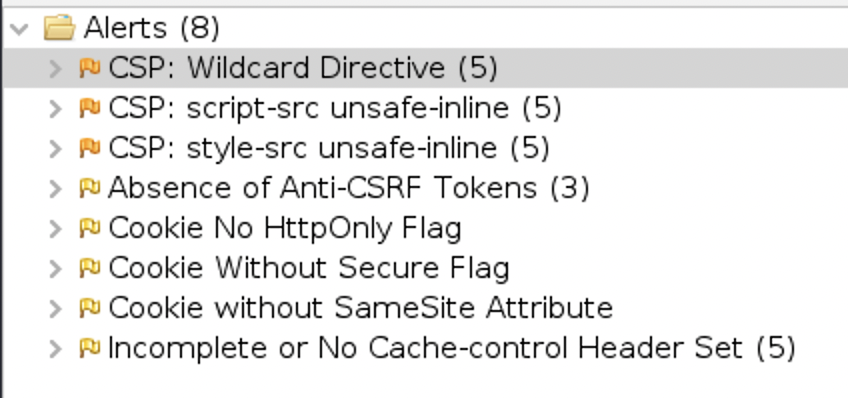
\includegraphics[scale=0.50]{images/security_risks_updated.png}
    \caption{Results from Zaproxy based on the newest version of our application.}
    \label{fig:Zaproxy_Updated}
\end{figure}


\subsection{Scaling \& Load balancing}

We have attempted to set up horizontal scaling via Docker Swarm, however we did not succeed in getting it to work completely. Our Swarm setup, which is currently on the \texttt{feature/swarm} git branch, can only run the MiniTwit application itself, so no monitoring nor logging. We believe this is due to issues with persistent storage, which is complicated to implement in a cluster setup.